
% ===========================================================================
% Title:
% ---------------------------------------------------------------------------
% to create Type I fonts type "dvips -P cmz -t letter <filename>"
% ===========================================================================
\documentclass[11pt]{article}       %--- LATEX 2e base
\usepackage{latexsym}               %--- LATEX 2e base
\usepackage{algorithm}
\usepackage{algpseudocode}
\usepackage{multirow}
\usepackage[table]{xcolor}
%---------------- Wide format -----------------------------------------------
\textwidth=6in \textheight=9in \oddsidemargin=0.25in
\evensidemargin=0.25in \topmargin=-0.5in
%--------------- Def., Theorem, Proof, etc. ---------------------------------
\newtheorem{definition}{Definition}
\newtheorem{theorem}{Theorem}
\newtheorem{lemma}{Lemma}
\newtheorem{corollary}{Corollary}
\newtheorem{property}{Property}
\newtheorem{observation}{Observation}
\newtheorem{fact}{Fact}
\newenvironment{proof}           {\noindent{\bf Proof.} }%
                                 {\null\hfill$\Box$\par\medskip}
%--------------- Figures ----------------------------------------------------
\usepackage{graphicx}
\usepackage{subcaption}
\newcommand{\includeFig}[3]      {\begin{figure}[htb] \begin{center}
                                 \includegraphics
                                 [width=4in,keepaspectratio] %comment this line to disable scaling
                                 {#2}\caption{\label{#1}#3} \end{center} \end{figure}}
                                 % usage: \includeFig{label}{file}{caption}

\usepackage{url}
\usepackage{parselines}
% ===========================================================================
\begin{document}
% ===========================================================================

% ############################################################################
% Title
% ############################################################################

\title{Parallelizing the Interpolation between Latent Space of Autoencoder
Networks}


% ############################################################################
% Author(s) (no blank lines !)
\author{
% ############################################################################
Tansin Jahan\\
School of Computer Science\\
Carleton University\\
Ottawa, Canada K1S 5B6\\
{\em tansinjahan@cmail.carleton.ca}
% ############################################################################
} % end-authors
% ############################################################################
\date{December 16, 2018}
\maketitle

% ############################################################################
% Abstract
% ############################################################################
\begin{abstract}
From early computing, faster execution of instructions is always been one of the major factors and because of that, faster logic devices and hardware improvements have been made to the machines. But focusing only on the hardware issues are not going to overcome this problem. Therefore, recent developments of parallel architecture combine both the hardware capability (ex- improvements on GPU) and implemented libraries (ex- CUDA framework and it's deep learning libraries such as cuDNN, Numba etc.) so that parallelism can be achieved easily. This project executes several matrix addition operations between the results of the convolutional neural network's layer and takes advantage of the CUDA platform to execute these operations inside GPU using multiple threads. By accessing GPU's shared memory, faster execution time has been achieved which compared to CPU is really significant. Though the result found by the CNN does not correspond to the expected output shape but the analysis of time differences between CPU and GPU was valuable and can lead to the possibilities of future research regarding parallelism inside a convolutional neural network.       
\end{abstract}

% ############################################################################
\section{Introduction} \label{intro}
% ############################################################################
The idea of parallel computing infers to execute more than one tasks simultaneously so that the complexity(ex- time, space etc.) in computation can be carried out smoothly. Though this is the simplest definition of parallel computing, in the real world, parallelization means a lot more than just handling the complexity in the computation of algorithms. With the development of Deep Learning Networks, parallel computing has become the essential choice for the implementation of these huge networks as it has to deal with lots of parameters.\newline

Parallelism can be introduced following different taxonomies of parallel architectures. According to Flynn's taxonomy, parallel architectures can be categorized as - Single Instruction Single Data(SISD), Multiple Instruction Single Data(MISD), Single Instructions Multiple Data(SIMD) and Multiple Instruction Multiple Data(MIMD) \cite{dr9}. In terms of memory parallelization, it can be divided into distributed and shared memory \cite{book1}.In addition with multicore and massive parallel clusters, GPU has become another predominant choice to aid in parallelism architecture. Using GPU's several core architectures, it becomes possible to run programs in parallel which provides unprecedented computational power for applications with large data. Nowadays the ubiquity and easy access to GPU through google cloud computing \cite{mis1} has made it more popular.\newline

So, I have divided the project into several groups such as - convolution of each input batches, loading data, and vector operations for different combinations of sample inputs. Then the time taken by each group is compared so that the parallelization can be introduced in such a way where the total runtime of the program can be optimum. Following the amount of input data, memory parallelization inside GPU to calculate vector operations between input samples seems more optimized and convenient as a parallelization technique.
For results, I tried to visually compare the time differences of GPU vs CPU in terms of different input sizes. And GPU performed 1.5x better than CPU as expected.\newline

In summary, for this project, several threads will be introduced to compute vector addition in CUDA so that the performance of the whole network can be improved. So, the rest of the paper is organized as follows - In Section~\ref{litrev}, we will review the relevant literature. Section~\ref{problemStatement} and~\ref{proposedSolution} will present the problem and it's proposed solution. In Section~\ref{expEval}, we will focus on the evaluation of experiment and computational time comparison between different approaches. At last, Section~\ref{concl} concludes the paper.


% ############################################################################
\section{Literature Review} \label{litrev}
% ############################################################################
\subsection{Object reconstruction using CNN} \label{subrev1}
With the recent development of Convolutional Neural Network, it has been used to solve several Computer Vision problem. For example, object detection or reconstruction from an input image, semantic information extraction from a scenario, object segmentation- these are all recent computer vision application where CNN has been used to produce a better result. Likewise, 3D reconstruction of an object is one of the Computer Vision problems and recently multiple approaches (ex: 3D-GAN, 3D-shapenets) has been proposed as a solution to the problem \cite{dr1}. In general, all these CNN models are considered as a generative model as it produces output based on a given input. But in terms of novelty, researchers are now more inclined to find something new rather than having just the same output as input. Following this, \textit{Alec Redford} in his paper \cite{radford2015unsupervised} experimented about using average mean vectors of input samples to produce new samples which gave very promising results. Another study recently shows that the interpolation between sample space and introducing noise vector can also produce good results for generative models. The experiment proposed a \textit{Generative Latent Optimization} model by exploiting properties of GANs: learning from large data, synthesizing visually-appealing samples, interpolating meaningfully between
samples, and performing linear arithmetic with noise vectors\cite{bojanowski2017optimizing}.\newline
\subsection{Current approaches for 3D object reconstruction } \label{subrev2}
Though most of these models chose a 2D image for their dataset but very few actually experimented with depth of an image. Previous work shows that given a depth image as input, the volumetric representation can be produced \cite{dr2}. Following these works, an approach to reconstruct the 3D voxelized object from a different viewpoint of one or more images of that object (i.e. single-view or multi-view) is proposed where the recurrent neural network has been used \cite{dr7}. In total 50,000 models is used to train and test the proposed network. Training the network with this large amount of data is really time-consuming and therefore introducing parallelism between the layers of the model can help to improve the performance of the network. \newline
\subsection{Parallelism in GPU} \label{subrev3}
GPU's parallel processor architecture has made it an essential choice for several applications where parallelism is needed. Such most common areas where GPU computing can be used are - Bioinformatics, Data Science, Analytics, and Databases, Defense and Intelligence, Machine Learning, Imaging and Computer Visions etc. \cite{samel2016gpu}. Using GPU's multithreaded processors, several threads can be introduced to perform matrix operations which are highly efficient for both graphics and general-purpose parallel computing applications \cite{nickolls2008scalable}. To execute programs in GPU written by high-level languages such as C, C++ or Python - CUDA provides a high-level interface by dividing CPU as host memory and GPU as device memory. In the CUDA programming model, the whole program is divided into several phases where the phase with data-parallelism is executed inside GPU using kernel functions and others implemented inside CPU. \cite{ryoo2008optimization}. In addition with interface CUDA also provides several GPU accelerated libraries such as - cuDNN for deep learning, NCCL for parallel algorithms, cuBLAS for linear algebra and math. These CUDA libraries are designed by Nvidia and 3x faster than CPU in terms of runtime \cite{mis2}. \newline
\begin{figure}[h]
\begin{center}
\includegraphics[scale=0.5]{autoencoder-architecture.png}
\caption{A simple autoencoder architecture}\cite{mis4} \label{autoencoder}
\end{center}
\end{figure}
For this project, I followed GPU shared memory parallelization to calculate 2D-vector addition operation inside the autoencoder network shown in figure \ref{autoencoder}. The implemented CNN for this project feeds on 3D volumes as input involving higher dimension(i.e. 32x32x32) and then reduces that into lower dimension \cite{dr8} which is called as latent space(also Z). In latent space, represented as Z vector, the input object has a minimum dimension with maximum features. From the lower dimension, the Z vector passes to deconvolution and therefore produces the same 3D volumes. But we can combine the Z vector of two input volumes to interpolate new points and give it to the decoder so that it can produce new 3D objects based on this interpolation. This interpolation of the Z vector (addition of two Z vectors) can be an overhead for the performance of the Autoencoder. Let us consider we have 50 inputs. Then for each input, we have to compare it with another 49 inputs and calculate interpolation each time. So, for 50 inputs the vector addition will be 50 x 50 which is in total 2500 times the addition of vectors.This calculation can take much time compared to the convolution and therefore we can parallelize this computation in GPU using Multithreading.\newline

% ############################################################################
\section{Problem Statement} \label{problemStatement}
% ############################################################################
From the studies of generative models, it is seen that most of these models focused on generating 2D images and does not take into account the depth or volume of any image. Moreover, it is also discussed in Section~\ref{subrev2} that, recent approaches for 3D object reconstruction using recurrent neural network \cite{dr7} or simple convolutional neural network \cite{dr2} produces the same output as input . Hence, the novelty gets suppressed by the regular design of generative models. This project intends to address this issue by leveraging generative models composition to introduce novelty in object reconstruction. Therefore the research question arises as following -     
\begin{enumerate}
\item Can we propose an interpolation technique inside convolutional neural network to change the expected output explicitly by means of matrix addition between two sample inputs?
\item As the interpolation technique involves matrix addition inside it, would shared memory parallelism be useful to reduce the total time of execution in terms of larger dataset?
\end{enumerate}
At each step, finding this interpolation between any two sample inputs might be an overhead if the matrix size becomes larger (example - 50,000 shapes of object). A general overview of time taken by GPU vs CPU for different sizes of matrix multiplication is shown in figure 2 \cite{latcharote2013high}. A CUDA platform for GPU programming will be an ideal option to speed up this computation.  
\begin{figure}[h]
\begin{center}
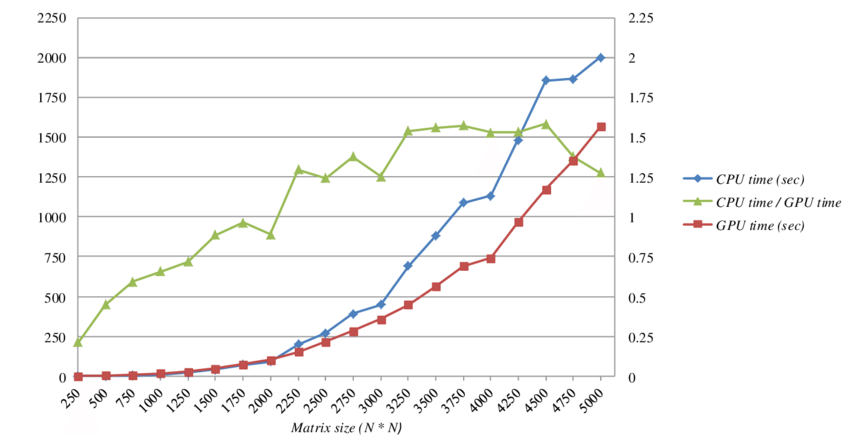
\includegraphics[scale=0.4]{time.png}
\caption{CPU vs GPU time for Matrix Multiplication}\cite{latcharote2013high}
\end{center}
\end{figure}
% ############################################################################
\section{Proposed Solution} \label{proposedSolution}
% ############################################################################
In this Section, we will discuss the approach taken to solve the research questions presented in Section~\ref{problemStatement}. So, subsection~\ref{algo} will present an algorithm to address research question of interpolation technique. Following that, subsection~\ref{partech} will describe the parallelization technique used for implementation of the algorithm specifically.
\subsection{Algorithm for interpolation} \label{algo}
The formal definition of Linear Interpolation is to generate new points given two known points. As for the autoencoder network of this project, Linear Interpolation would mean to interpolate new vector(i.e. latent space or \textbf{z}) by adding two other vectors produced by two known shapes. Then we will provide this new \textbf{z} to the network so that it can create new shape between the range of the given vectors. Generally these vectors can be of any shape but for the simplicity we created it as a 2D matrix. So the algorithm is as follows -


\begin{algorithm}
  \caption {Algorithm to generate new \textbf{z} as latent space for Autoencoder} \label{algoZ}
  \begin{algorithmic}[1]
      \For{\texttt{i = first input shape}}
      	\For{\texttt{j = second input shape}}
      	 \State{\texttt{z1 = z vector for i}}
      	 \State{\texttt{z2 = z vector for j}}
      	 \For{\texttt{t = 0 to 1}}
      	  \State{\texttt{newz = (1-t) * z1 + t * z2}}
      	  \State{\texttt{run decoder network}}
      	  \State{\texttt{t = t + 0.1}}
      	 \EndFor
        \EndFor						
      \EndFor
    
  \end{algorithmic}
\end{algorithm}

\subsection{Parallelism} \label{partech}
The innermost loop of our algorithm contains vector addition and scalar multiplication between range of [0,1]. This computation can be executed in parallel manner by leveraging the power of GPU. For clarification, the dimension of both z1 and z2 is [8 by 8]. GPU provided by NVIDIA has now become the most common choice for high performance parallel computing application. And CUDA architecture takes this advantage of GPU computing to run highly parallelized program  \cite{mis3}.  
NVIDIA CUDA architecture provides  two interfaces - i) A device-level programming interface and ii) A language integration programming interface. Through second interface, we can write programs using high-level language(ex- C,C++,Python) and C Runtime for CUDA automatically handles setting up the GPU and executing the compute functions \cite{mis3}. Another important objective of CUDA is that it divides the execution of program between \textbf{host} and \textbf{device} which represents comsecutively \textbf{CPU} and \textbf{GPU}. Multiple threads can be initialized inside CPU and can be sent to GPU for executing in parallel manner. Threads can be grouped together in a block and mutiple blocks build together grids of thread blocks. Beacuse of the hardware chip configuration, shared memory is much faster than local and global memory. And each thread block is allocated this shared memory, so all threads in the block can access to the same shared memory. 

\begin{figure}
\centering
\begin{subfigure}{.5\textwidth}
  \centering
  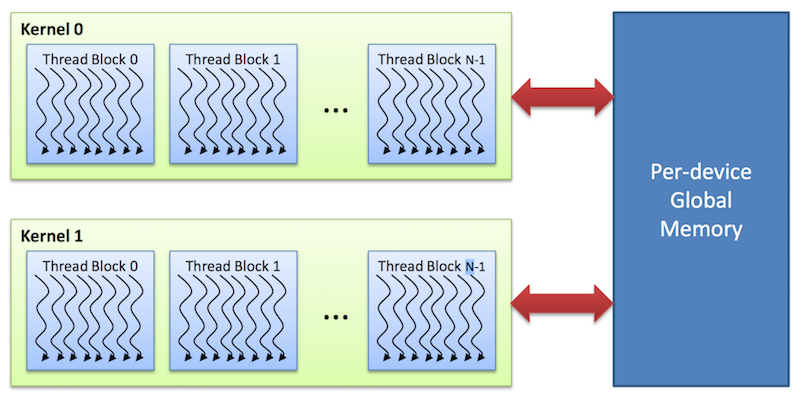
\includegraphics[width=1.0\linewidth]{globalmemory.png}
  \caption{Thread blocks in Kernel}
  \label{fig:sub1}
\end{subfigure}%
\begin{subfigure}{.4\textwidth}
  \centering
  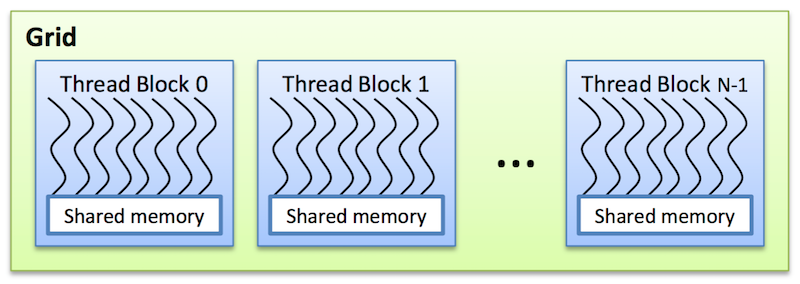
\includegraphics[width=1.0\linewidth]{threadgrid.png}\newline
  \caption{Shared memory access of all threads in each block}
  \label{fig:sub2}
\end{subfigure}
\caption{CUDA parallel programming architecture}
\label{fig:test}
\end{figure}


% ############################################################################
\section{Experimental Evaluation} \label{expEval}
% ############################################################################

For this experiment, one particular object(i.e. chair ) has been chosen as dataset. But it can also be extended for other objects. Firstly, Section~\ref{expEval} will focus on explaining dataset and the configuration of CNN. Then parallel thread architecture used for the experiment will be discussed followed by the time comparison between CPU and GPU for total input shapes.
\subsection{Dataset and GPU configuration} \label{data}
As I mentioned in Section~\ref{subrev3}, 50 different shapes of chair in total has been used for this experiment which has been downloaded from ShapeNet \cite{shapenet2015}. Among those, 40 shapes has been used as training data and 10 shapes has been used for testing data. Each of these shapes has dimension of [32 x 32 x 32]\newline
The GPU used here is NVIDIA Titan V with 8 virtual cores. Total RAM space is 30GB and the version of OS is UBUNTU 16.04
\subsection{CNN and training} \label{cnn}
The CNN model named Autoencoder used here consists of \textbf{Encoder}(for convolution) and \textbf{Decoder}(for deconvolution) and both has exactly 3 layers to convolute over the input object. Table~\ref{table1} indicates the output structure after convolution in each of the layers. So, encoder takes an input volume of [32 x 32 x 32 x 1] and produce an output shape of [2 x 2 x 2 x 8] which is designated as \textbf{z}(i.e. latent space). This \textbf{z} then passed to the kernel where interpolation takes on and \textbf{newz} returned to the decoder which later on gives the output based on the changes made to that \textbf{z} vector. 
\begin{table}[H]
\caption{The highlighted output of encoder [2 x 2 x 2 x 8] represents \textbf{z} and reshaped into [8 x 8] to perform vector operation conveniently inside kernel. No feature is lost or modified in this reshape operation as dimension remains unchanged. After interpolation \textbf{z} again reshaped into [2 x 2 x 2 x 8] to follow the model architecture and feed to the Decoder.}
\begin{center}
\begin{tabular}{ |c|c|c|c|c| } 
\hline
Encoder & Interpolation & Decoder \\
\hline
32 x 32 x 32 x 1 & \multirow{4}{15em}{[8 x 8] + [8 x 8] \\ newz = [8 x 8] \\ reshaped into = [2 x 2 x 2 x 8]} & \cellcolor[HTML]{FDEE00} 2 x 2 x 2 x 8 \\ 
%\hline
16 x 16 x 16 x 32 & & 8 x 8 x 8 x 16 \\ 
%\hline
8 x 8 x 8 x 16 & & 16 x 16 x 16 x 32 \\
%\hline
\cellcolor[HTML]{FDEE00} 2 x 2 x 2 x 8 & & 32 x 32 x 32 x 1 \\
\hline
\end{tabular}
\end{center}
\label{table1}
\end{table}
\subsection{Threads and results comparison } \label{vec}
To utilize GPU's computational power, 4 blocks of thread has been initialized. The dimension of threads are [4 x 4]. The kernel function takes two input vectors(\textbf{z1} and \textbf{z2}), one output vector(\textbf{newz}) and a scalar value(\textbf{t} as number inside given interpolation range) as arguments for calculation. In figure \ref{threadfig}, implemented threads and blocks architecture for this experiment is shown.

\begin{figure}[h]
\centering
\begin{subfigure}{.5\textwidth}
  \centering
  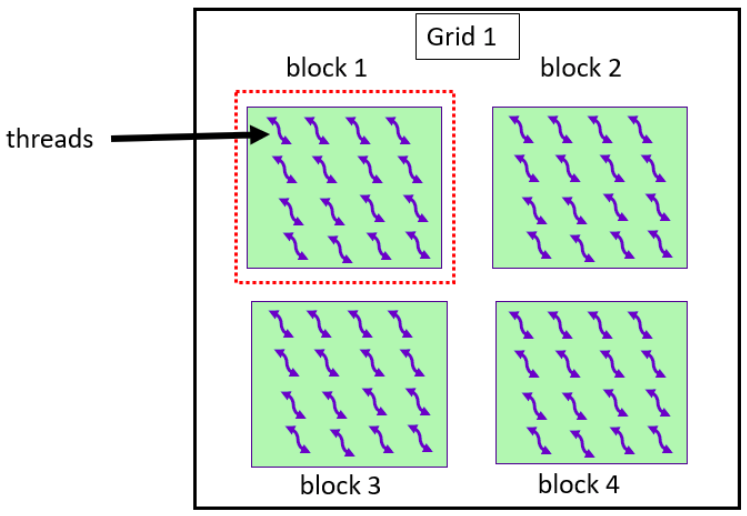
\includegraphics[width=0.9\linewidth]{par.png}
  \caption{Threads architecture for the experiment}\label{threadfig}
\end{subfigure}%
\begin{subfigure}{.5\textwidth}
  \centering
  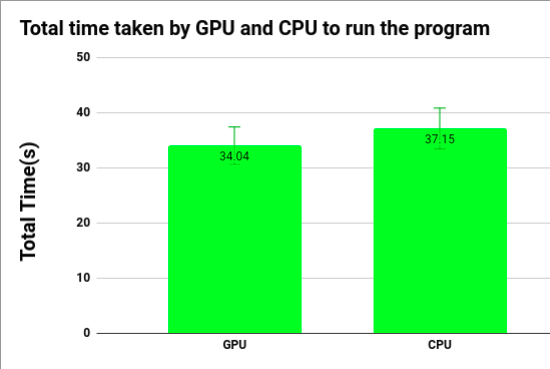
\includegraphics[width=0.9\linewidth]{cpu-gpu.png}
  \caption{Time comparison between CPU and GPU}\label{comp}
  \label{fig:sub2}
\end{subfigure}
\caption{First subfigure \ref{threadfig} shows how many threads are implemented and subfigure \ref{comp} represents the total time taken by CPU and GPU to complete the program using shared memory}\label{fig:test}
\end{figure}

\subsection{CPU vs GPU analysis } \label{CPU-GPU}
Two versions of the program has been implemented. In the first version, threads performed the vector addition using global memory and in another one using shared memory. The time for each of the execution has been compared. Table \ref{memorytable} represents time taken by different operations inside the program. It is observed from Table \ref{memorytable} that for input size 2, shared memory took  0.17s to complete the vector operation where global memory took 0.24s. As for CNN running time, it remains same for both CPU and GPU which is 11 seconds. \newline

Another CPU version of the program is also implemented to compare with GPU. The results are described in Table \ref{memorytable} and Table \ref{input-time}. For input size 2, total time taken by GPU is 35.04 seconds whereas, CPU took 37.15 seconds. So, GPU speedup over CPU is 1.06 seconds which is not very significant.    But surprisingly, when the input size grows, the differences also became visible significantly. For example, table \ref{input-time} shows that for 50 inputs, GPU takes only 0.09s but CPU took 0.9s. We can see from line graph \ref{analysis} that, GPU tends to take less time as input grows and become steady in opposed to CPU. In summary, we can claim that GPU is not certainly robust enough for computation in terms of smaller input. But when the input size is large enough than GPU will surely outperform CPU by providing faster computation time.     

\begin{table}[h]
  \centering
  \caption{Time differences on GPU in terms of Shared and Global memory} \label{memorytable}   
    	\begin{tabular}{|c|c|c|c|}
        	\hline
        	Different Methods & GPU(s) & CPU(s)\\
        	\hline
        	Vectoradd time(shared) & 0.17 & 0.0017 \\
        	\hline
       		Vectoradd time(global) & 0.24 & 0.0017 \\
        	\hline
        	CNN run time & 11 & 11 \\
        	\hline
        	Total program run time & 35.04 & 37.15 \\
        	\hline
    	\end{tabular}
\end{table}
\begin{table}[h]
\centering
  \caption{GPU and CPU time differences vs input size} \label{input-time}
  \begin{tabular}{c|c|c|}
        	\cline{2-3}
             & \multicolumn{2}{|c|}{Time(s)}\\
        	\hline
        	\multicolumn{1}{|c|}{Input size} & GPU & CPU \\
        	\hline
        	\multicolumn{1}{|c|}{2} & 0.17 & 0.0017 \\
        	\hline
        	\multicolumn{1}{|c|}{10} & 0.15 & 0.0024 \\
        	\hline
        	\multicolumn{1}{|c|}{20} & 0.12 & 0.034 \\
        	\hline
        	\multicolumn{1}{|c|}{30} & 0.10 & 0.54 \\
        	\hline
        	\multicolumn{1}{|c|}{40} & 0.09 &	0.78 \\
        	\hline
        	\multicolumn{1}{|c|}{50} & 0.09 & 0.9 \\
        	\hline
    \end{tabular}
\end{table}

\begin{figure}[h]
\begin{center}
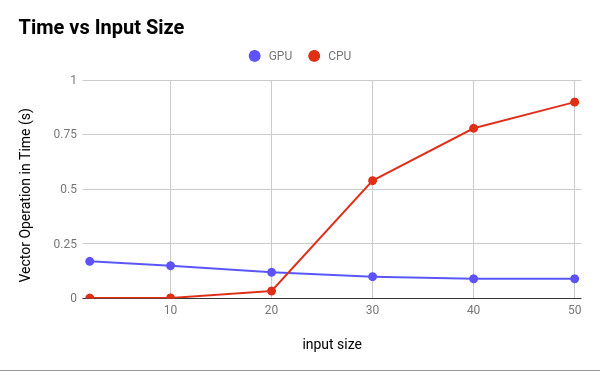
\includegraphics[scale=0.5]{chart-para.png} 
\caption{The variance of GPU and CPU time is shown in compared to the input sizes}\label{analysis}
\end{center}
\end{figure}
\subsection{Autoencoder output } \label{output}
In this section, we will discuss the results provided by the \textbf{Autoencoder} network after interpolation. As preliminary results, it can be seen from figure \ref{autooutput} that the output shape niether biased to any of the input shape nor it corresponds to a new shape as expected from the network. There can be several issues involved such as networks learning parameters, range of interpolated values etc. As future work, these issue can be certainly focused on which will help to detect the problem associated with the output.
\begin{figure}[h]
\begin{center}
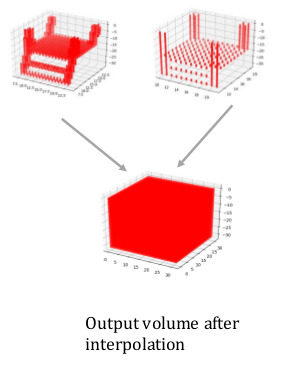
\includegraphics[scale=0.7]{1.png} 
\caption{Output shape from two given input shape through interpolation inside latent space}\label{autooutput}
\end{center}
\end{figure}

% ############################################################################
\section{Conclusion} \label{concl}
% ############################################################################
To keep compute time minimized for any task is really important. Nowadays recent improvements on GPU's are especially focused to maintain this overhead. GPU's are always preferred for deep learning as CNN and it's parameter computation can be complex sometimes. The approaches taken in this project by leveraging GPU's shared memory parallelism contributes to improving the runtime of the program despite involving 6 layers of Convolutional Neural Network. In addition, the project also takes the input of 3D volumes and tries to make some new shape out of it is not very common for most of the CNN. Moreover,  analysis like - global or shared memory time comparison, CPU or GPU time differences in terms of input sizes has given very interesting insightful which can lead to further research in deep learning to minimize the time complexity of heavy networks.\newline
For future work, several other parallelism approaches can also be taken and compared with this one to find a better solution. And other CUDA deep learning libraries such as cuDNN can be used to implement the CNN. So that it can help to improve the overall performance of the network. To conclude, GPU parallelism supports to minimize runtime of the program if the computational operation is large enough. Otherwise, CPU might outperform GPU and GPU's computability might not be utilized properly.


% ############################################################################
% Bibliography
% ############################################################################
\bibliographystyle{plain}
\bibliography{my-bibliography}     %loads my-bibliography.bib

% ============================================================================
\end{document}
% ============================================================================
